\documentclass[11pt,a4paper]{article}
\usepackage[utf8]{inputenc}
\usepackage[T1]{fontenc}
\usepackage[spanish]{babel}
\usepackage{amsmath,amssymb}
\usepackage{graphicx}
\usepackage{booktabs}
\usepackage{float}
\usepackage{geometry}
\geometry{margin=2.5cm}
\usepackage{hyperref}
\hypersetup{colorlinks=true, linkcolor=blue, urlcolor=blue, citecolor=blue}

\title{\textbf{Práctica 3.1 / Experimento 1: Estudio de la Corrosión}\\[0.3em]\large Efecto del pH, Diagramas de Pourbaix y Análisis de Esfuerzos}
\author{Grado en Ingeniería Química -- RMDM}
\date{\today}

\begin{document}

\maketitle

\section{Objetivos}
\begin{itemize}
    \item Identificar en los Diagramas de Pourbaix las condiciones de potencial y pH en las que un metal está protegido o sufre corrosión.
    \item Evaluar experimentalmente la velocidad de corrosión de electrodos de Zinc ($\text{Zn}$) y Cobre ($\text{Cu}$) a diferentes valores iniciales de pH ($\text{pH}_0 = 4$ y $\text{pH}_0 = 9$).
    \item Ubicar los datos medidos de pH en los Diagramas de Pourbaix para justificar los regímenes de corrosión activa o pasivación.
\end{itemize}

\section{Fundamento Teórico y Reacciones (Apartado 3.1.3 c)}

\subsection{Corrosión del Zinc ($\text{Zn}$)}
\begin{itemize}
    \item \textbf{Medio Ácido ($\text{pH}_0 = 4$)}:
    \begin{align}
        \text{Anódica:} \quad & \text{Zn(s)} \rightarrow \text{Zn}^{2+}(\text{aq}) + 2e^- \quad (E^0 = -0.763 \text{ V}) \\
        \text{Catódica:} \quad & 2\text{H}^+ + 2e^- \rightarrow \text{H}_2(\text{g}) \quad \text{y/o} \quad \text{O}_2 + 4\text{H}^+ + 4e^- \rightarrow 2\text{H}_2\text{O}
    \end{align}
    El consumo de protones ($\text{H}^+$) provoca un incremento constante del pH hacia la neutralidad. La velocidad de corrosión es elevada debido a la inestabilidad de las capas pasivas en medio ácido.

    \item \textbf{Medio Básico ($\text{pH}_0 = 9$)}:
    Según el \textbf{Diagrama de Pourbaix}, el zinc a pH $8.5$--$10.5$ entra en su \textbf{zona de pasivación}, formando hidróxido o película insoluble de óxido:
    \begin{equation}
        \text{Zn}^{2+} + 2\text{OH}^- \rightarrow \text{Zn(OH)}_2(\text{s})
    \end{equation}
    Esta capa pasivante recubre la superficie del metal y disminuye la velocidad de corrosión en más de un orden de magnitud.
\end{itemize}

\subsection{Corrosión del Cobre ($\text{Cu}$)}
El cobre presenta un potencial estándar de reducción positivo ($E^0_{\text{Cu}^{2+}/\text{Cu}} = +0.34\text{ V}$), por lo que \textbf{no reduce espontáneamente los protones} $\text{H}^+$ para producir $\text{H}_2$. Su corrosión requiere oxígeno disuelto como agente despolarizante catódico:
\begin{align}
    \text{Anódica:} \quad & \text{Cu(s)} \rightarrow \text{Cu}^{2+}(\text{aq}) + 2e^- \\
    \text{Catódica:} \quad & \text{O}_2 + 4\text{H}^+ + 4e^- \rightarrow 2\text{H}_2\text{O} \quad (\text{ácido}) \quad \text{o} \quad \text{O}_2 + 2\text{H}_2\text{O} + 4e^- \rightarrow 4\text{OH}^- \quad (\text{básico})
\end{align}
A pH 4 la corrosión es moderada/baja y a pH 9 es casi nula por la formación de óxidos pasivantes pasivos ($\text{Cu}_2\text{O} / \text{CuO}$).

% \section{Diagramas de Pourbaix y Puntos Experimentales}
% (Desactivado temporalmente)

\section{Resultados Experimentales (Experimento 3.1)}

\begin{table}[H]
\centering
\caption{Electrodo de Zinc (Zn) - $\text{pH}_{\text{inicial}} = 4$}
\label{tab:zn_ph4}
\begin{tabular}{cccccccc}
\toprule
t (días) & t (h) & Masa (g) & Masa (\%) & Pérdida (mg) & v\_acum (mg/h) & v\_int (mg/h) & pH \\
\midrule
0.0000 & 0.0000 & 7.7700 & 100.00 & 0.0000 & 0.0000 & 0.0000 & 4.1000 \\
0.9380 & 22.5100 & 7.7332 & 99.5264 & 36.8000 & 1.6347 & 1.6347 & 4.6700 \\
1.9480 & 46.7500 & 7.6889 & 98.9562 & 81.1000 & 1.7347 & 1.8276 & 5.2200 \\
2.9480 & 70.7500 & 7.6482 & 98.4324 & 121.80 & 1.7215 & 1.6958 & 5.6300 \\
5.8650 & 140.76 & 7.6098 & 97.9382 & 160.20 & 1.1381 & 0.5485 & 6.5800 \\
6.0750 & 145.80 & 7.6077 & 97.9112 & 162.30 & 1.1132 & 0.4167 & 6.8600 \\
\bottomrule
\end{tabular}
\end{table}

\begin{table}[H]
\centering
\caption{Electrodo de Zinc (Zn) - $\text{pH}_{\text{inicial}} = 9$}
\label{tab:zn_ph9}
\begin{tabular}{cccccccc}
\toprule
t (días) & t (h) & Masa (g) & Masa (\%) & Pérdida (mg) & v\_acum (mg/h) & v\_int (mg/h) & pH \\
\midrule
0.0000 & 0.0000 & 8.3209 & 100.00 & 0.0000 & 0.0000 & 0.0000 & 9.1900 \\
0.9380 & 22.5100 & 8.3147 & 99.9255 & 6.2000 & 0.2754 & 0.2754 & 9.1500 \\
1.9480 & 46.7500 & 8.3116 & 99.8882 & 9.3000 & 0.1989 & 0.1279 & 9.5400 \\
2.9480 & 70.7500 & 8.3082 & 99.8474 & 12.7000 & 0.1795 & 0.1417 & 9.3400 \\
5.8650 & 140.76 & 8.3013 & 99.7644 & 19.6000 & 0.1392 & 0.0986 & 9.4000 \\
6.0750 & 145.80 & 8.2997 & 99.7452 & 21.2000 & 0.1454 & 0.3175 & 9.6000 \\
\bottomrule
\end{tabular}
\end{table}

\begin{table}[H]
\centering
\caption{Electrodo de Cobre (Cu) - $\text{pH}_{\text{inicial}} = 4$}
\label{tab:cu_ph4}
\begin{tabular}{cccccccc}
\toprule
t (días) & t (h) & Masa (g) & Masa (\%) & Pérdida (mg) & v\_acum (mg/h) & v\_int (mg/h) & pH \\
\midrule
0.0000 & 0.0000 & 9.6686 & 100.00 & 0.0000 & 0.0000 & 0.0000 & 4.0900 \\
0.9380 & 22.5100 & 9.6583 & 99.8935 & 10.3000 & 0.4575 & 0.4575 & 4.1200 \\
1.9480 & 46.7500 & 9.6584 & 99.8945 & 10.2000 & 0.2182 & -0.0041 & 4.4300 \\
2.9480 & 70.7500 & 9.6574 & 99.8842 & 11.2000 & 0.1583 & 0.0417 & 4.3500 \\
5.8650 & 140.76 & 9.6554 & 99.8635 & 13.2000 & 0.0938 & 0.0286 & 4.3800 \\
6.0750 & 145.80 & 9.6548 & 99.8573 & 13.8000 & 0.0947 & 0.1190 & 4.3800 \\
\bottomrule
\end{tabular}
\end{table}

\begin{table}[H]
\centering
\caption{Electrodo de Cobre (Cu) - $\text{pH}_{\text{inicial}} = 9$}
\label{tab:cu_ph9}
\begin{tabular}{cccccccc}
\toprule
t (días) & t (h) & Masa (g) & Masa (\%) & Pérdida (mg) & v\_acum (mg/h) & v\_int (mg/h) & pH \\
\midrule
0.0000 & 0.0000 & 9.7060 & 100.00 & 0.0000 & 0.0000 & 0.0000 & 9.1700 \\
0.9380 & 22.5100 & 9.7048 & 99.9876 & 1.2000 & 0.0533 & 0.0533 & 9.1200 \\
1.9480 & 46.7500 & 9.7046 & 99.9856 & 1.4000 & 0.0299 & 0.0083 & 9.5200 \\
2.9480 & 70.7500 & 9.7046 & 99.9856 & 1.4000 & 0.0198 & -0.0000 & 9.5400 \\
5.8650 & 140.76 & 9.7024 & 99.9629 & 3.6000 & 0.0256 & 0.0314 & 9.3400 \\
6.0750 & 145.80 & 9.7020 & 99.9588 & 4.0000 & 0.0274 & 0.0794 & - \\
\bottomrule
\end{tabular}
\end{table}


\section{Representación Gráfica}

\begin{figure}[H]
    \centering
    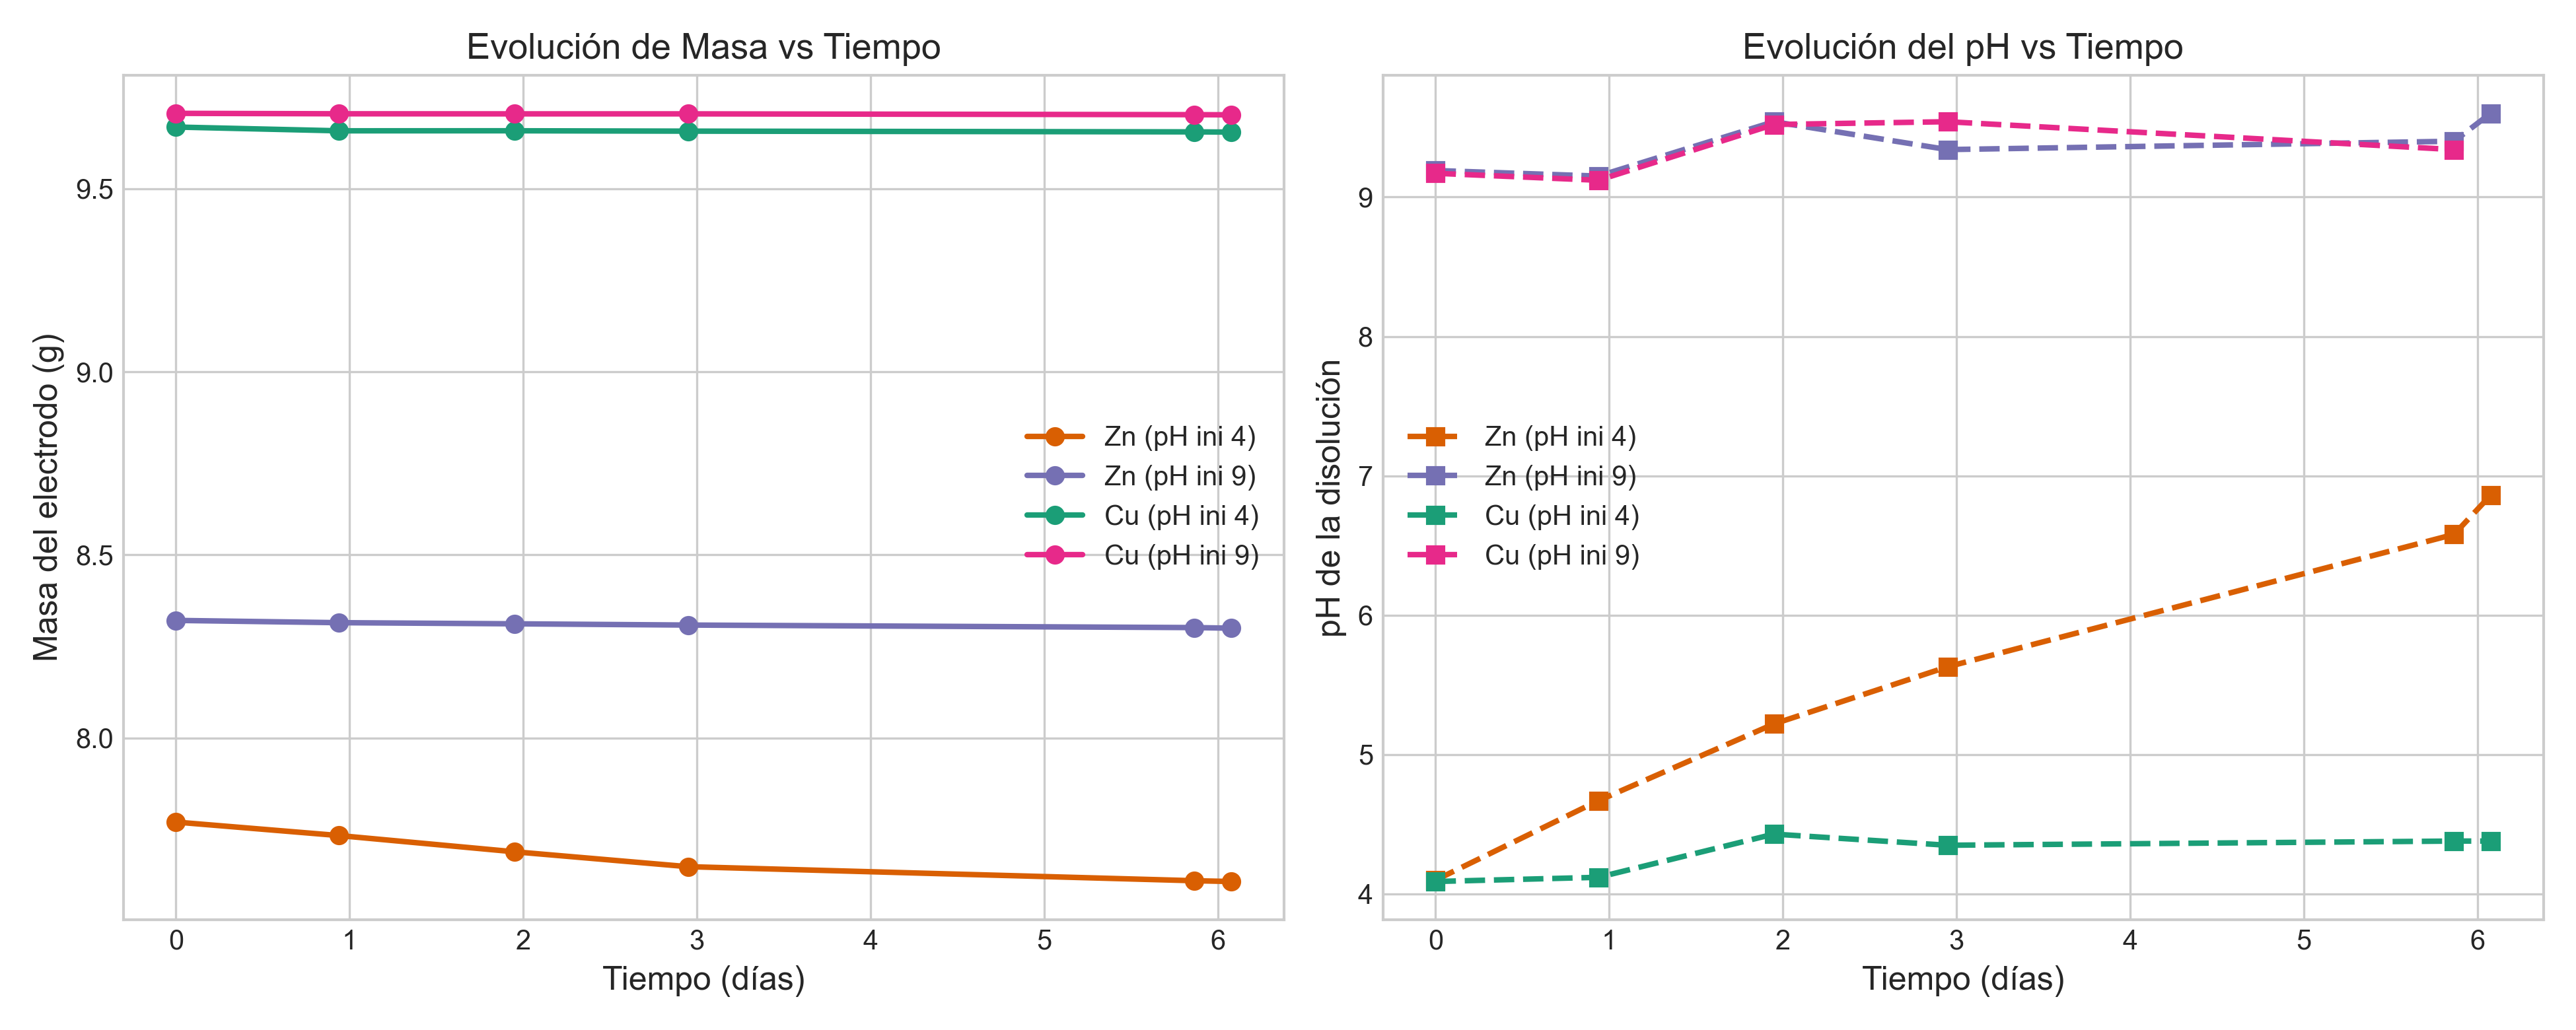
\includegraphics[width=0.95\textwidth]{resultados_practica_corrosion/exp_3_1_masa_y_pH.png}
    \caption{Evolución de la masa del electrodo y del pH en función del tiempo.}
    \label{fig:masa_pH}
\end{figure}

\begin{figure}[H]
    \centering
    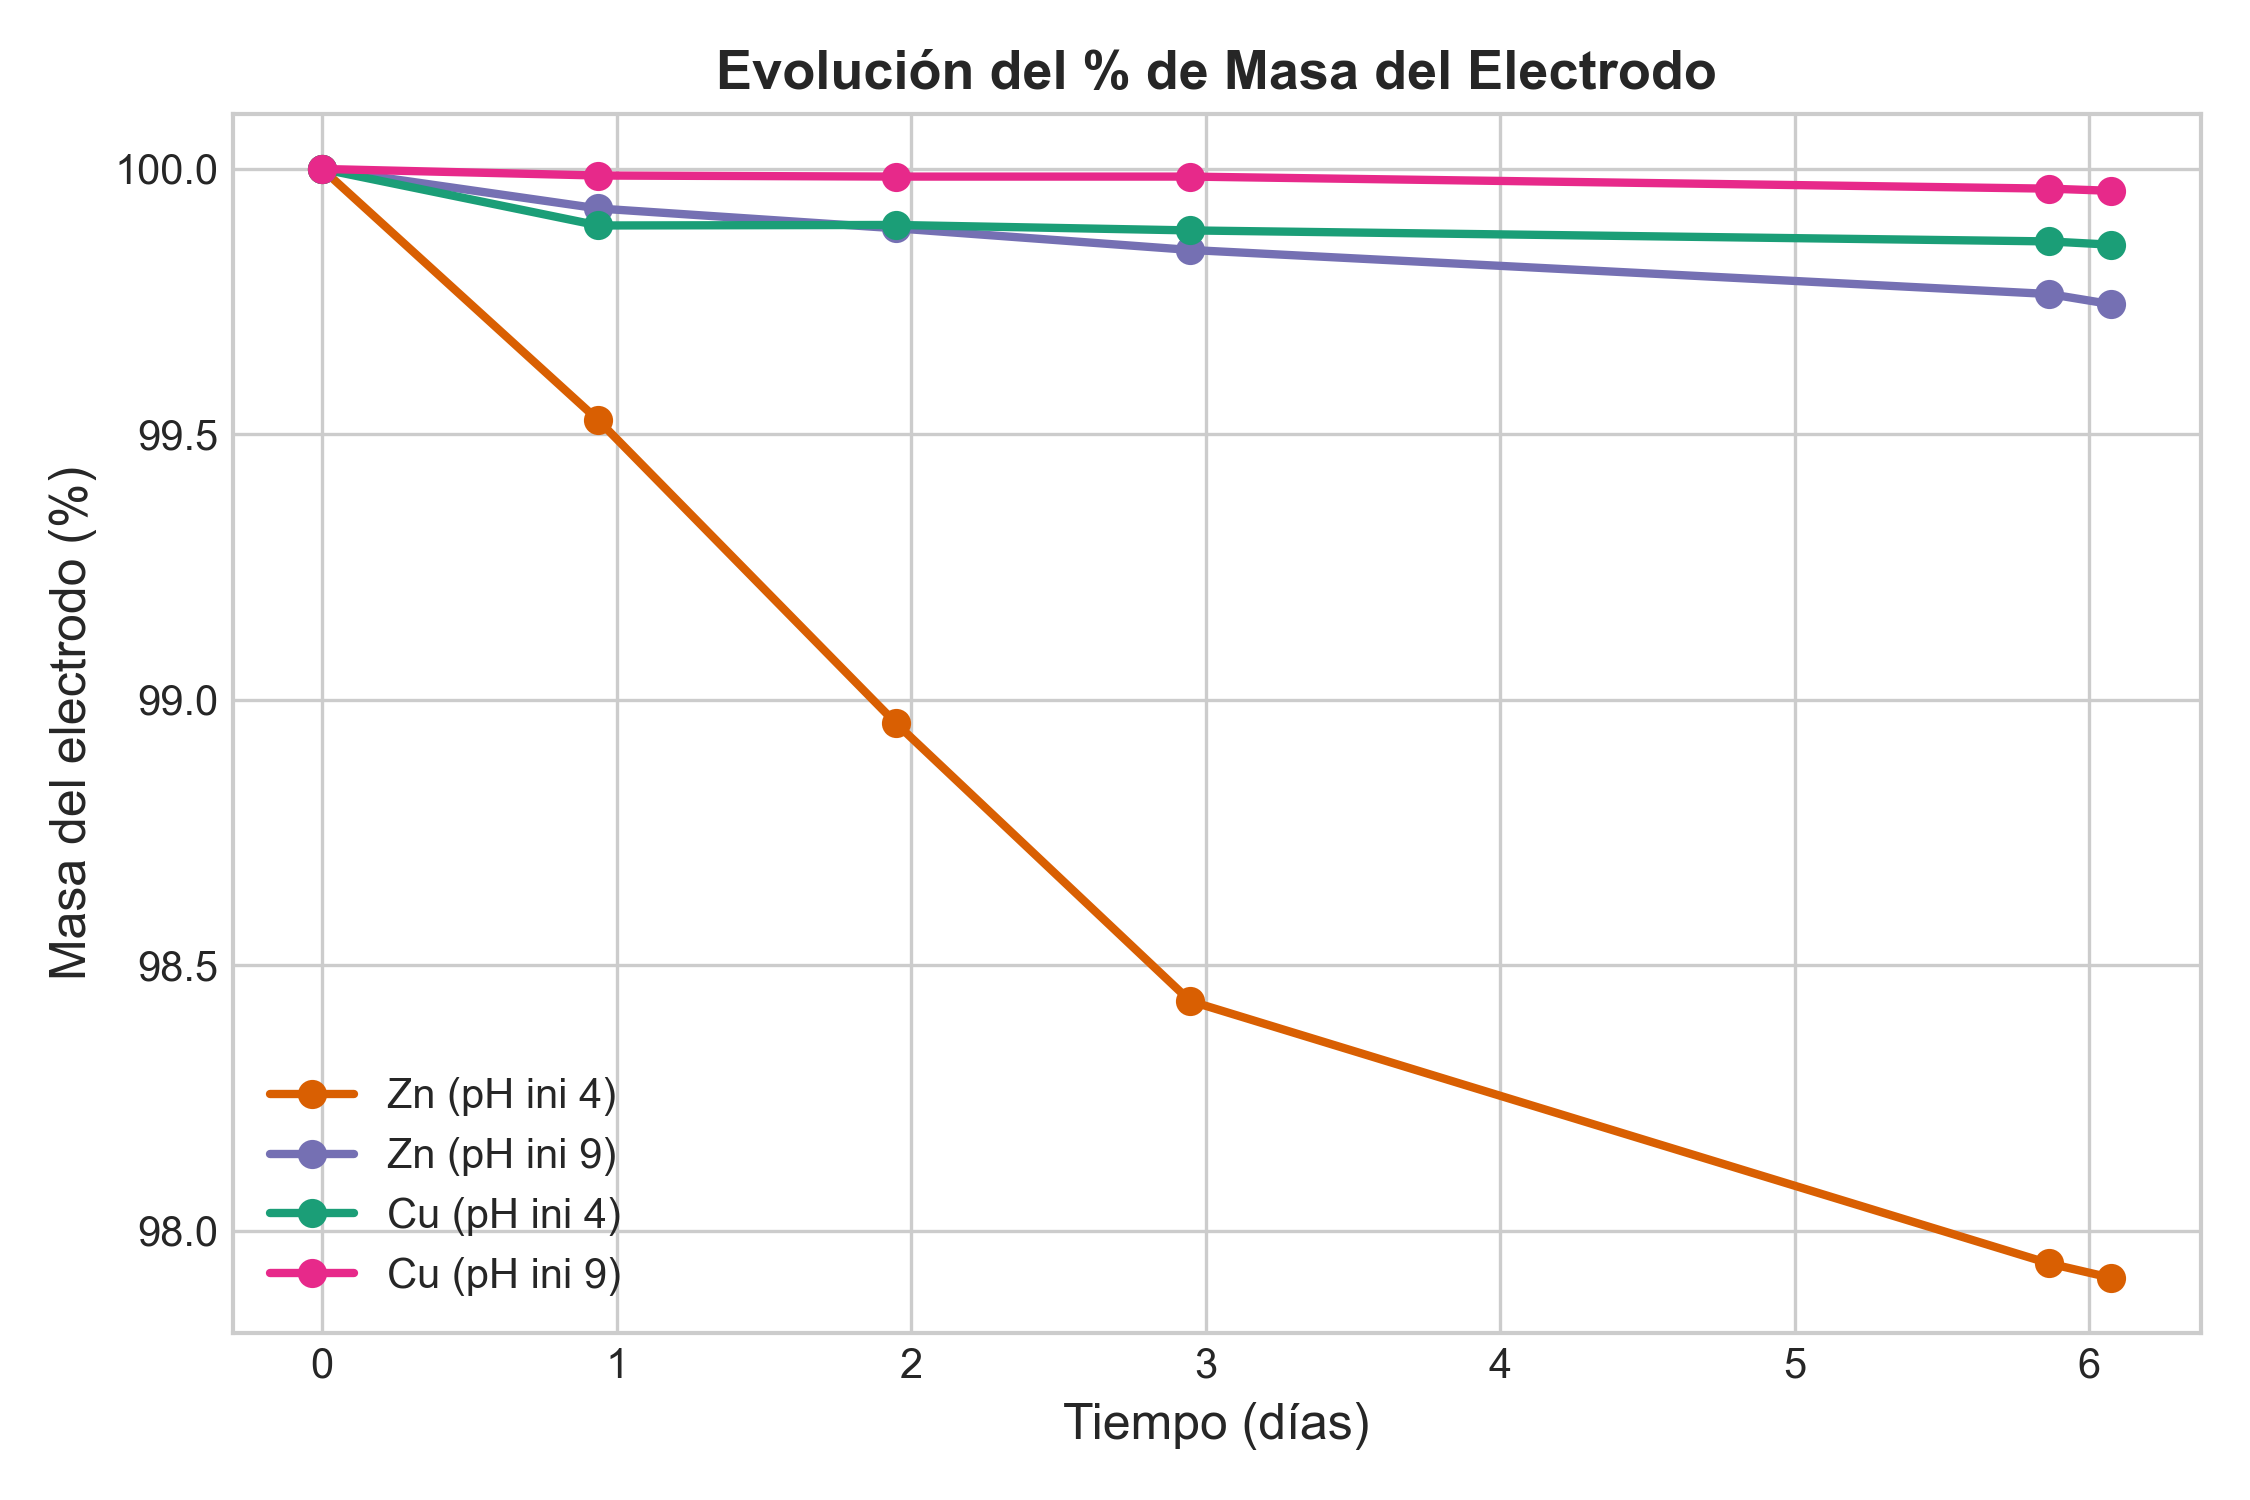
\includegraphics[width=0.75\textwidth]{resultados_practica_corrosion/exp_3_1_porcentaje_masa.png}
    \caption{Porcentaje de masa restante del electrodo respecto a la inicial.}
    \label{fig:porcentaje_masa}
\end{figure}

\begin{figure}[H]
    \centering
    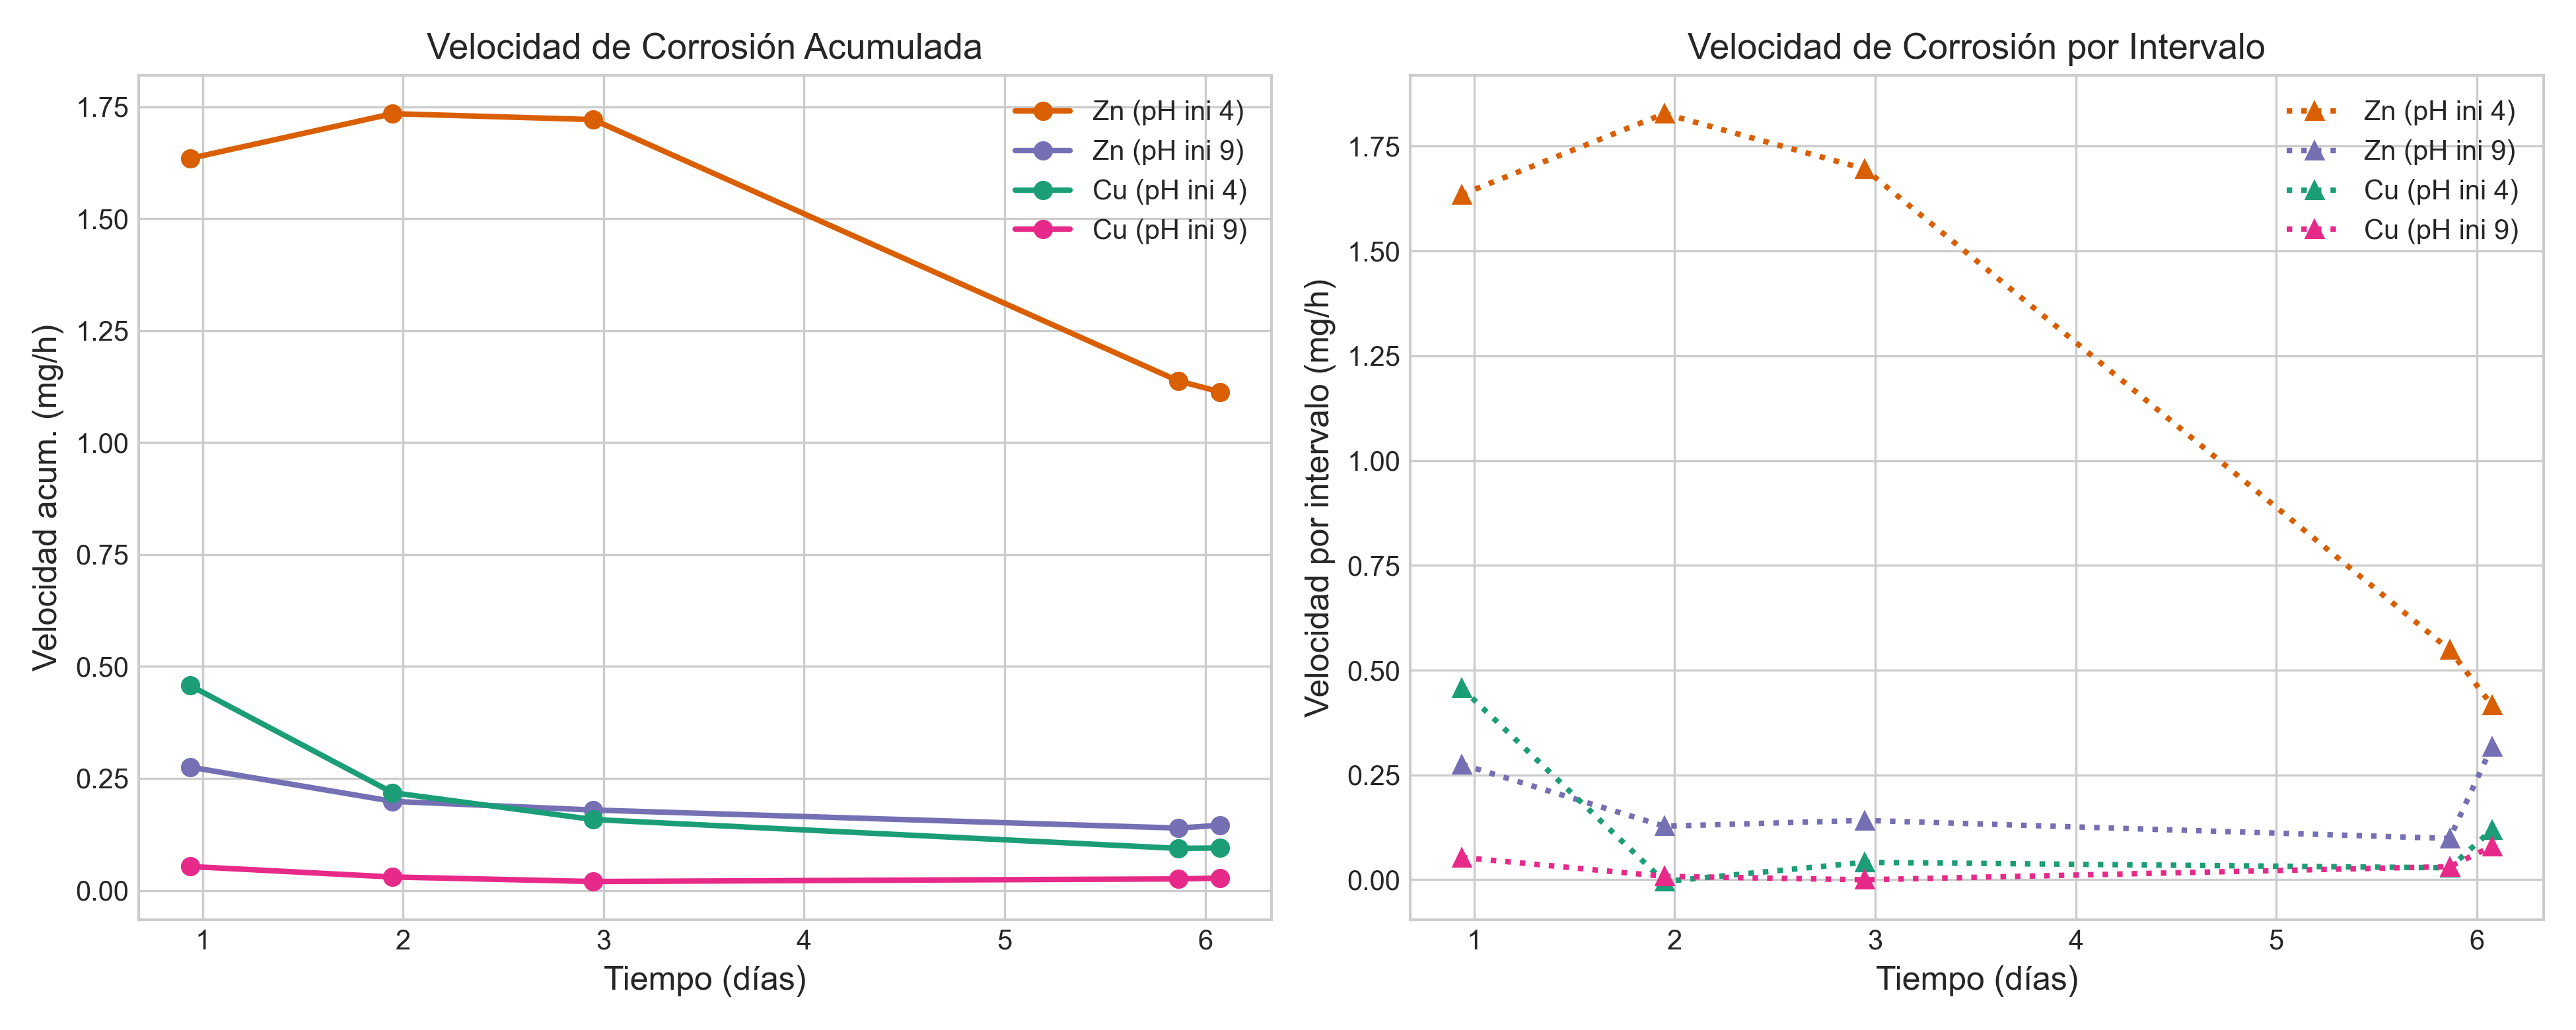
\includegraphics[width=0.95\textwidth]{resultados_practica_corrosion/exp_3_1_velocidad_corrosion.png}
    \caption{Velocidad de corrosión acumulada y por intervalo en función del tiempo.}
    \label{fig:v_corrosion}
\end{figure}

\section{Resultados del Experimento 3.2 (Subgrupo A: Corrosión bajo Esfuerzos)}

\begin{table}[H]
\centering
\caption{Probeta de acero NO taladrada en HCl 2N}
\label{tab:no_taladrada}
\begin{tabular}{ccccccc}
\toprule
t (min) & t (h) & Masa (g) & Masa (\%) & Pérdida (mg) & v\_acum (mg/h) & v\_int (mg/h) \\
\midrule
0.0000 & 0.0000 & 8.6398 & 100.00 & 0.0000 & 0.0000 & 0.0000 \\
5.0000 & 0.0830 & 8.6396 & 99.9977 & 0.2000 & 2.4000 & 2.4000 \\
15.0000 & 0.2500 & 8.6385 & 99.9850 & 1.3000 & 5.2000 & 6.6000 \\
25.0000 & 0.4170 & 8.6371 & 99.9687 & 2.7000 & 6.4800 & 8.4000 \\
35.0000 & 0.5830 & 8.6364 & 99.9606 & 3.4000 & 5.8286 & 4.2000 \\
50.0000 & 0.8330 & 8.6356 & 99.9514 & 4.2000 & 5.0400 & 3.2000 \\
65.0000 & 1.0830 & 8.6333 & 99.9248 & 6.5000 & 6.0000 & 9.2000 \\
80.0000 & 1.3330 & 8.6329 & 99.9201 & 6.9000 & 5.1750 & 1.6000 \\
107.00 & 1.7830 & 8.6297 & 99.8831 & 10.1000 & 5.6636 & 7.1111 \\
132.00 & 2.2000 & 8.6293 & 99.8785 & 10.5000 & 4.7727 & 0.9600 \\
145.00 & 2.4170 & 8.6278 & 99.8611 & 12.0000 & 4.9655 & 6.9231 \\
165.00 & 2.7500 & 8.6279 & 99.8623 & 11.9000 & 4.3273 & -0.3000 \\
185.00 & 3.0830 & 8.6270 & 99.8518 & 12.8000 & 4.1514 & 2.7000 \\
205.00 & 3.4170 & 8.6252 & 99.8310 & 14.6000 & 4.2732 & 5.4000 \\
225.00 & 3.7500 & 8.6245 & 99.8229 & 15.3000 & 4.0800 & 2.1000 \\
245.00 & 4.0830 & 8.6230 & 99.8056 & 16.8000 & 4.1143 & 4.5000 \\
\bottomrule
\end{tabular}
\end{table}

\begin{table}[H]
\centering
\caption{Probeta de acero TALADRADA (con concentración de esfuerzos) en HCl 2N}
\label{tab:taladrada}
\begin{tabular}{ccccccc}
\toprule
t (min) & t (h) & Masa (g) & Masa (\%) & Pérdida (mg) & v\_acum (mg/h) & v\_int (mg/h) \\
\midrule
0.0000 & 0.0000 & 8.3728 & 100.00 & 0.0000 & 0.0000 & 0.0000 \\
5.0000 & 0.0830 & 8.3719 & 99.9893 & 0.9000 & 10.8000 & 10.8000 \\
15.0000 & 0.2500 & 8.3702 & 99.9689 & 2.6000 & 10.4000 & 10.2000 \\
25.0000 & 0.4170 & 8.3689 & 99.9534 & 3.9000 & 9.3600 & 7.8000 \\
35.0000 & 0.5830 & 8.3675 & 99.9367 & 5.3000 & 9.0857 & 8.4000 \\
50.0000 & 0.8330 & 8.3659 & 99.9176 & 6.9000 & 8.2800 & 6.4000 \\
65.0000 & 1.0830 & 8.3641 & 99.8961 & 8.7000 & 8.0308 & 7.2000 \\
80.0000 & 1.3330 & 8.3625 & 99.8770 & 10.3000 & 7.7250 & 6.4000 \\
107.00 & 1.7830 & 8.3589 & 99.8340 & 13.9000 & 7.7944 & 8.0000 \\
132.00 & 2.2000 & 8.3568 & 99.8089 & 16.0000 & 7.2727 & 5.0400 \\
145.00 & 2.4170 & 8.3565 & 99.8053 & 16.3000 & 6.7448 & 1.3846 \\
165.00 & 2.7500 & 8.3542 & 99.7779 & 18.6000 & 6.7636 & 6.9000 \\
185.00 & 3.0830 & 8.3530 & 99.7635 & 19.8000 & 6.4216 & 3.6000 \\
205.00 & 3.4170 & 8.3517 & 99.7480 & 21.1000 & 6.1756 & 3.9000 \\
225.00 & 3.7500 & 8.3509 & 99.7384 & 21.9000 & 5.8400 & 2.4000 \\
245.00 & 4.0830 & 8.3508 & 99.7372 & 22.0000 & 5.3878 & 0.3000 \\
\bottomrule
\end{tabular}
\end{table}


\begin{figure}[H]
    \centering
    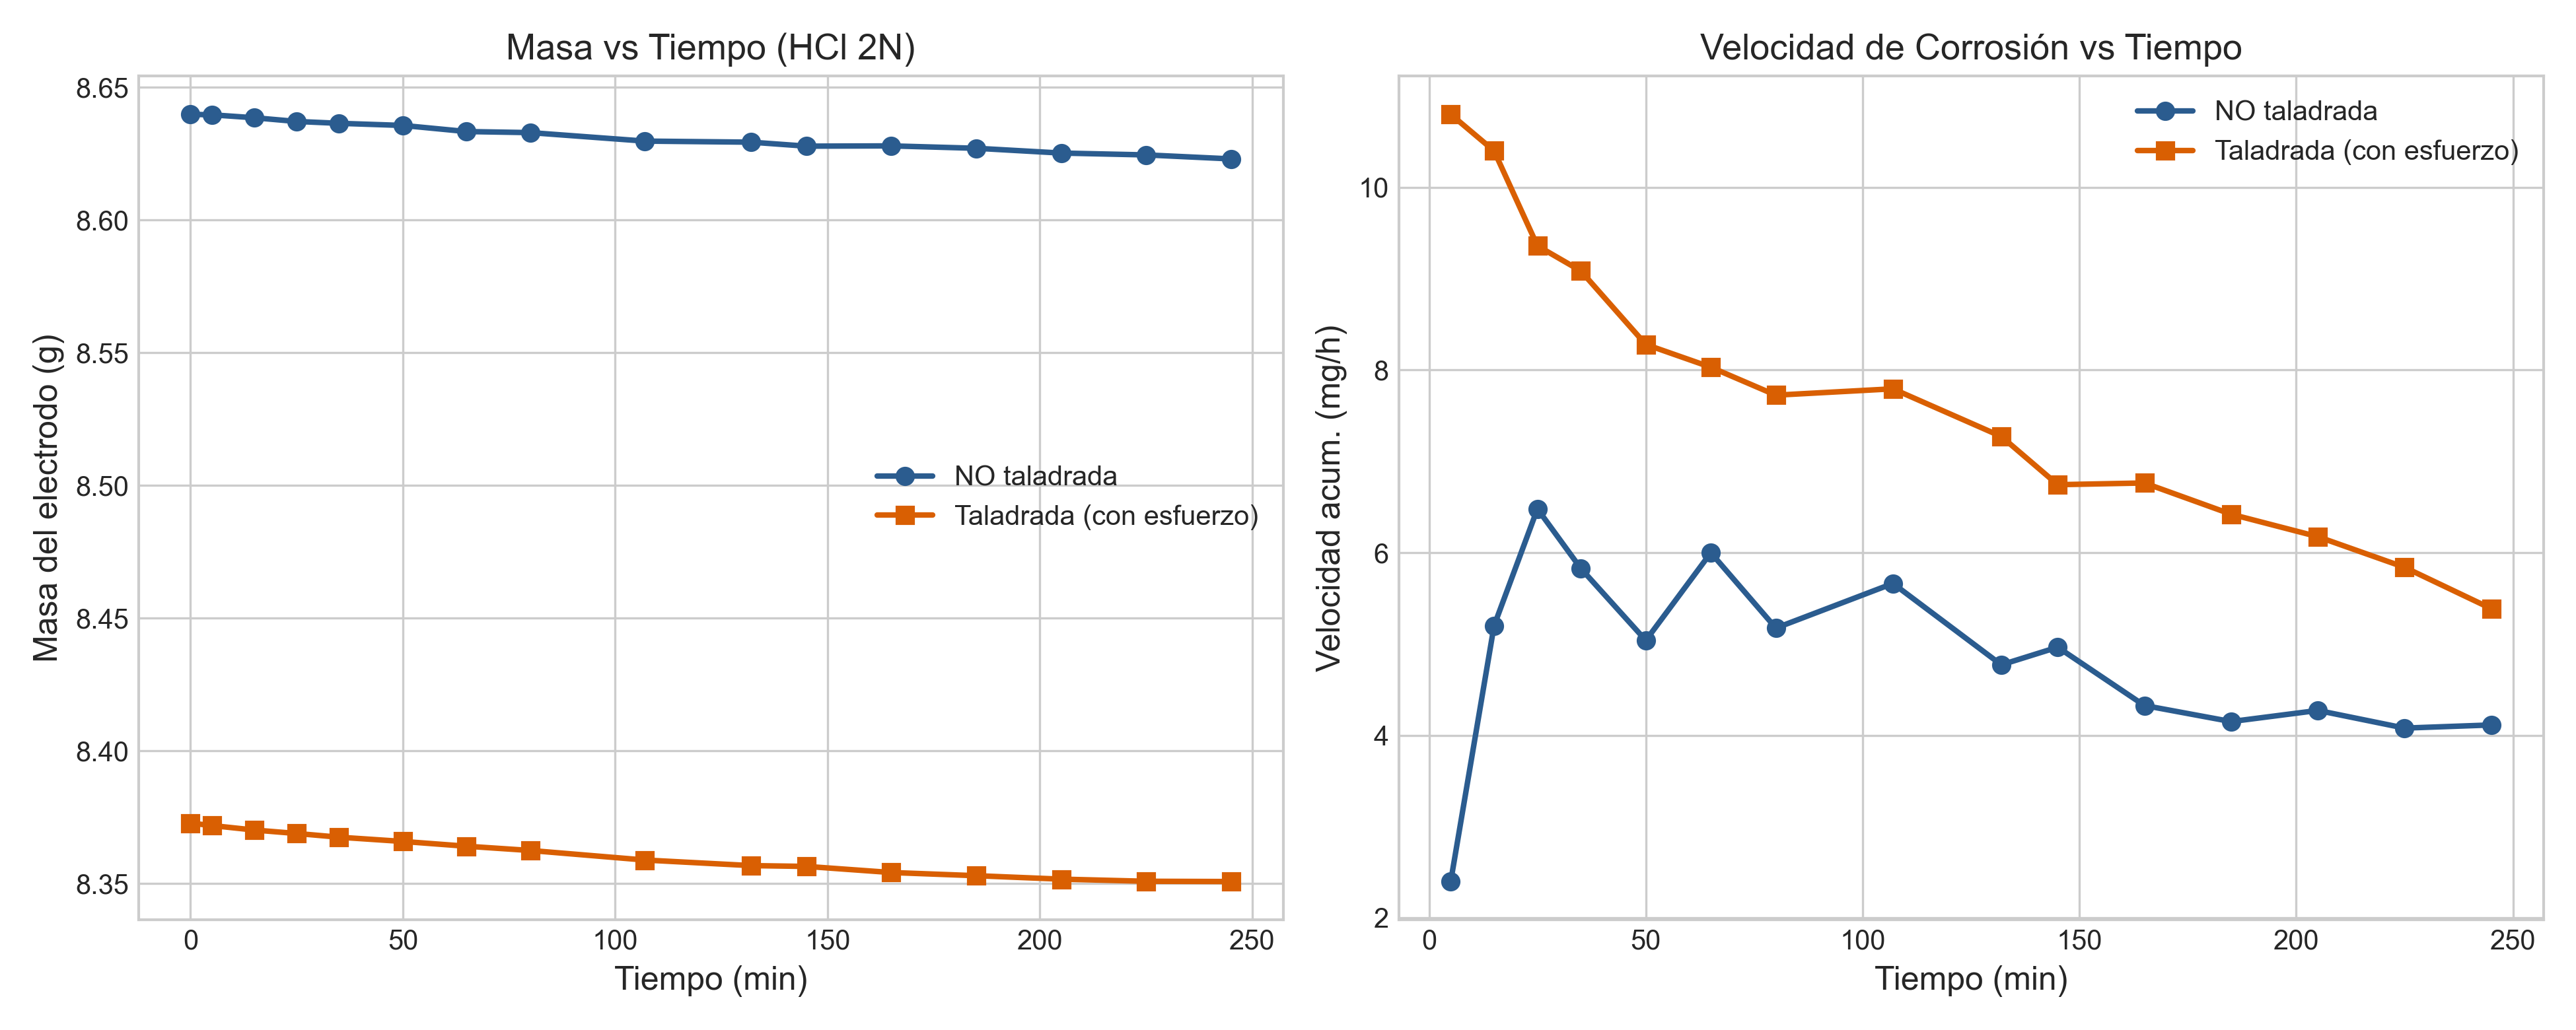
\includegraphics[width=0.95\textwidth]{resultados_practica_corrosion/exp_3_2_esfuerzos.png}
    \caption{Efecto de la concentración de esfuerzos en la masa y velocidad de corrosión.}
    \label{fig:esfuerzos}
\end{figure}

\end{document}
